\problemset{Теория вероятностей и математическая статистика}
\problemset{Индивидуальное домашнее задание №2}

% Команда ниже задает "название" или слово, которое будет
% отображаться вместо proof или "доказательство"
% поскольку у нас в ИДЗ задачи - то нужно слово "Решение"
\renewcommand*{\proofname}{Решение}

%%%%%%%%%%%%%% ЗАДАНИЕ №1 %%%%%%%%%%%%%%
%% Условие задания №1
\begin{problem}
Распределение случайной величины $\xi $ задано таблицей:
\begin{center}
\begin{table}[h!]
    \centering
    \begin{tabular}{|c|c|c|c|c|c|c|}
        \hline
        $\xi$ & -1 & 0 & 1 & 2 & 3 & $\sum$ \\
        \hline
        $\Prob$ & 1/8 & 1/4 & 1/8 & 1/8 & 3/8 & 1 \\
        \hline
    \end{tabular}
\end{table}
\end{center}
Вычислить $\Expect\xi $, $\Variance\xi $, $\Entropy\xi $ (в натах). Вычислить распределение $ \eta = \cos(\pi\xi/2)$. Построить графики функций распределений $ F_{\xi}(x)$ и $ F_{\eta}(y)$.
\end{problem}

%% Решение задания №1
\begin{proof}
$\supp\xi = \{-1, 0, 1, 2, 3\}$. $\xi$ - дискретная случайная величина (ДСВ). Тогда ее математическое ожидание можно найти по формуле:
\[
\Expect\xi = \sum_{i: p_i > 0} a_i\cdot p_i = -1\cdot\frac{1}{8} + 0\cdot\frac{1}{4} + 1\cdot\frac{1}{8} + 2\cdot\frac{1}{8} + 3\cdot\frac{3}{8} = \frac{11}{8} = 1.375
\]
Для нахождения $\Variance\xi$ воспользуемся свойством: $\Variance\xi = \Expect\xi^2 - (\Expect\xi)^2$; а также формулой для начального момента k-го порядка ДСВ: $\Expect\xi^k = \sum_{i: p_i > 0} a_i^k\cdot p_i$.\\
Тогда:
\begin{gather*}
\Expect\xi^2 = \sum_{i: p_i > 0} a_i^2\cdot p_i = 1\cdot\frac{1}{8} + 0\cdot\frac{1}{4} + 1\cdot\frac{1}{8} + 4\cdot\frac{1}{8} + 9\cdot\frac{3}{8} = \frac{33}{8} = 4\frac{1}{8}\\
\Variance\xi = \Expect\xi^2 - (\Expect\xi)^2 = \frac{33}{8} - \frac{121}{64} = \frac{143}{64} \approx 2.2343
\end{gather*}
Энтропию в натах найдем по известной формуле:
\[
\Entropy\xi = -\sum_{i: p_i > 0} p_i\ln p_i \approx 1.4942 \text{ нат}
\]
$\eta = \cos(\pi\xi/2)$ и $\supp\xi = \{-1, 0, 1, 2, 3\}$.
\begin{gather*}
    \eta(-1) = 0\\
    \eta(0) = 1\\
    \eta(1) = 0\\
    \eta(2) = -1\\
    \eta(3) = 0\\
\end{gather*}
Значит $\supp\eta = \{-1, 0, 1\}$.
\begin{center}
\begin{table}[h!]
    \centering
    \begin{tabular}{|c|c|c|c|c|}
        \hline
        $\eta$ & -1 & 0 & 1 & $\sum$\\
        \hline
        $\Prob$ & 1/8 & 5/8 & 2/8 & 1\\
        \hline
    \end{tabular}
\end{table}
\end{center}
Пояснение к таблице:
\begin{figure}[h!]
    \centering
    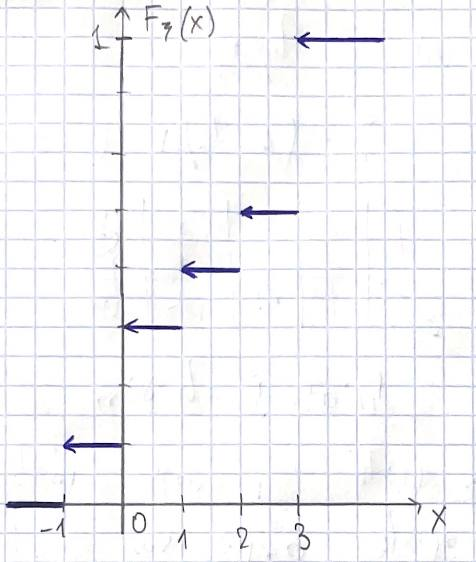
\includegraphics[width=0.5\linewidth]{1.jpg}
    \caption{}
    \label{fig:enter-label}
\end{figure}
\begin{figure}[h!]
    \centering
    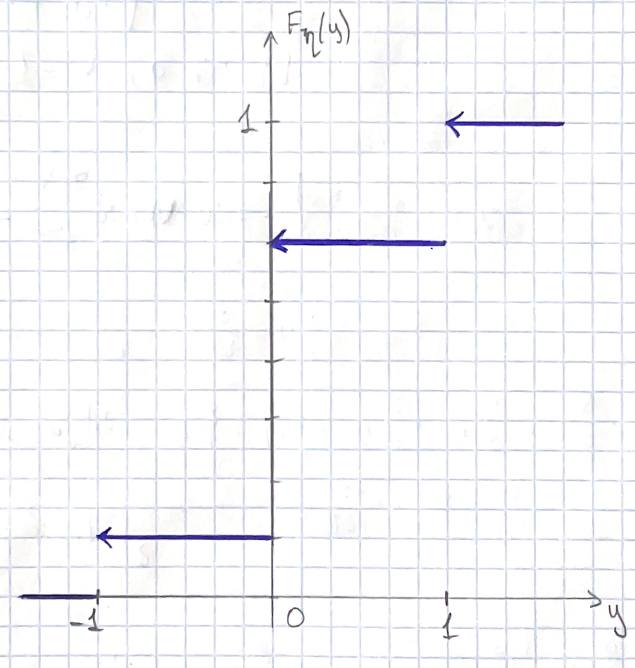
\includegraphics[width=0.5\linewidth]{2.jpg}
    \caption{}
    \label{fig:enter-label}
\end{figure}
\begin{gather*}
    \Prob(\eta = -1) = \Prob(\xi = 2) = \frac{1}{8}\\
    \Prob(\eta = 0) = \Prob(\xi = -1) +  \Prob(\xi = 1) + \Prob(\xi = 3)= \frac{5}{8}\\
    \Prob(\eta = 1) = \Prob(\xi = 0) = \frac{1}{4} = \frac{2}{8}\\
\end{gather*}
Теперь найдем $ F_{\xi}(x)$ и $ F_{\eta}(y)$:
\[ 
F_{\xi}(x) = \begin{cases} 
          0, & x\in (-\infty; -1] \\
          \frac{1}{8}, & x\in (-1; 0] \\
          \frac{3}{8}, & x\in (0; 1] \\
          \frac{4}{8}, & x\in (1; 2] \\
          \frac{5}{8}, & x\in (2; 3] \\
          1, & x\in (3; \infty) \\
       \end{cases}
F_{\eta}(y) = \begin{cases} 
          0, & x\in (-\infty; -1] \\
          \frac{1}{8}, & x\in (-1; 0] \\
          \frac{6}{8}, & x\in (0; 1] \\
          1, & x\in (1; \infty) \\
       \end{cases}
\]
Их графики на рисунках 1 и 2 соответственно.
{\it Ответ:}\\
$\Expect\xi$ = 1.375, $\Variance\xi$ = 2.2343, $\Entropy\xi$ = 1.4942 нат\\

\end{proof}

%%%%%%%%%%%%%% ЗАДАНИЕ №2 %%%%%%%%%%%%%%
%% Условие задания №2
\begin{problem}
Дана плотность распределения абсолютно непрерывной случайной величины $\xi$:
\[ 
p_{\xi}(x) = \begin{cases} 
          C, & x\in [3; 6] \\
          3C, & x\in (6; 8] \\
          0, & \text{в отс. сл.} \\
       \end{cases}
\]
Вычислить С, $\Expect\xi $, $\Variance\xi $, $\Entropy\xi $ (в натах). Вычислить распределение $\eta = \xi^4$. Построить графики функций распределений $ F_{\xi}(x)$ и $ F_{\eta}(y)$.
\end{problem}

%% Решение задания №2
\begin{proof}
Воспользуемся свойством плотности распределения абсолюнто непрерывной случайной величины (АНСВ). Интеграл от плотности по всей числовой прямой должен равняться 1. Тогда:
\[
\int\limits_{-\infty}^{\infty}p_{\xi}(x)dx = C\int\limits_3^6dx + 3C\int\limits_6^8dx = 9C = 1 \Rightarrow C = \frac{1}{9}
\]
И тогда:
\[ 
p_{\xi}(x) = \begin{cases} 
          \frac{1}{9}, & x\in [3; 6] \\
          \frac{1}{3}, & x\in (6; 8] \\
          0, & \text{в отс. сл.} \\
       \end{cases}
\]
Найдем математическое ожидание по известной формуле для АНСВ:
\[
\Expect\xi = \int\limits_{-\infty}^{\infty}x\cdot p_{\xi}(x)dx = \frac{1}{9}\int\limits_3^6xdx + \frac{1}{3}\int\limits_6^8xdx = \frac{27}{18} + \frac{28}{6} = \frac{37}{6} \approx 6.1667
\]
Найдем дисперсию по известному свойству:
\begin{gather*}
\Expect\xi^2 = \int\limits_{-\infty}^{\infty}x^2\cdot p_{\xi}(x)dx = \frac{1}{9}\int\limits_3^6x^2dx + \frac{1}{3}\int\limits_6^8x^2dx = \frac{189}{27} + \frac{296}{9} = \frac{359}{9}\\
\Variance\xi = \Expect\xi^2 - (\Expect\xi)^2 = \frac{359}{9} - \frac{1369}{36} = \frac{67}{36} \approx 1.8611\\
\end{gather*}
Найдем энтропию по известной формуле:
\[
\Entropy\xi = -\int\limits_{-\infty}^{\infty}p_{\xi}(x)\cdot\ln(p_{\xi}(x))dx = -\left(\int\limits_3^6\frac{1}{9}\ln\frac{1}{9}dx + \int\limits_6^8\frac{1}{3}\ln\frac{1}{3}dx\right) \approx 1.4648 \text{нат}
\]
$\supp\xi = [3;8], \eta = \xi^4 \Rightarrow \supp\eta = [81;4096] = [81;1296]\cup[1296;4096]$.\\
1) $\eta\in [81;1296]\Rightarrow\xi\in [3;6]$ и $\eta$ монотонно возрастает.\\
\[
\begin{cases}
    g_1(x) = x^4\\
    g_1^{-1}(y) = \sqrt[4]y\\
\end{cases}
\]
Тогда $p_{1\eta}(y) = \frac{1}{36}\cdot\frac{1}{\sqrt[4]y^3}$.\\
2) $\eta\in [1296; 4096]\Rightarrow\xi\in [6;8]$ и $\eta$ монотонно возрастает.\\
\[
\begin{cases}
    g_2(x) = x^4\\
    g_2^{-1}(y) = \sqrt[4]y\\
\end{cases}
\]
Тогда $p_{2\eta}(y) = \frac{1}{12}\cdot\frac{1}{\sqrt[4]y^3}$.\\
Итого:
\[ 
p_{\eta}(y) = \begin{cases} 
          \frac{1}{36}\cdot\frac{1}{\sqrt[4]y^3}, & y\in [81; 1296] \\
          \frac{1}{12}\cdot\frac{1}{\sqrt[4]y^3}, & x\in (1296; 4096] \\
          0, & \text{в отс. сл.} \\
       \end{cases}
\]
Найдем $ F_{\xi}(x)$ и $ F_{\eta}(y)$:
\begin{figure}[h!]
    \centering
    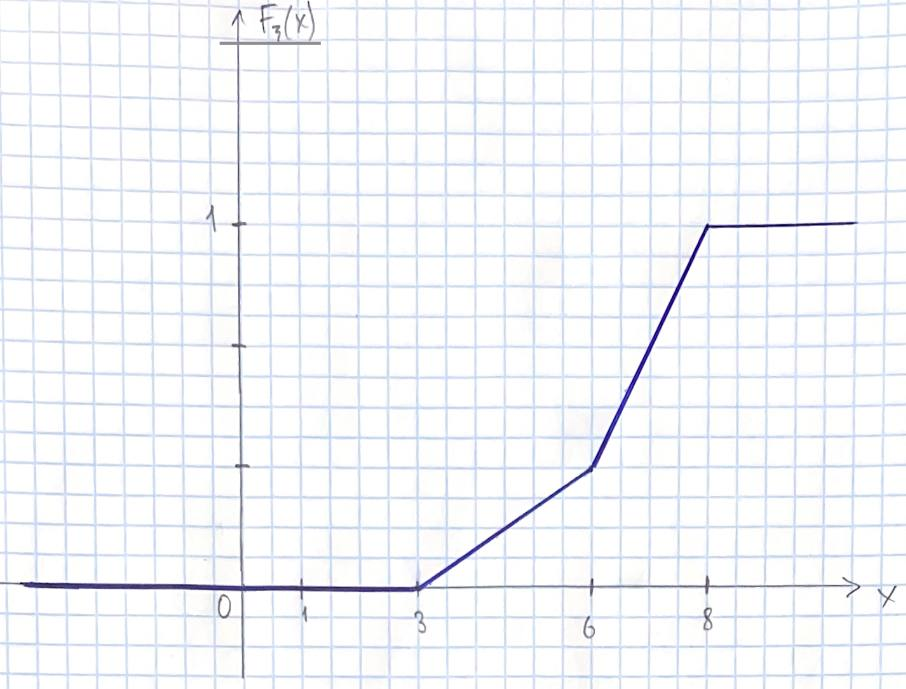
\includegraphics[width=0.5\linewidth]{3.jpg}
    \caption{}
    \label{fig:enter-label}
\end{figure}
\begin{figure}[h!]
    \centering
    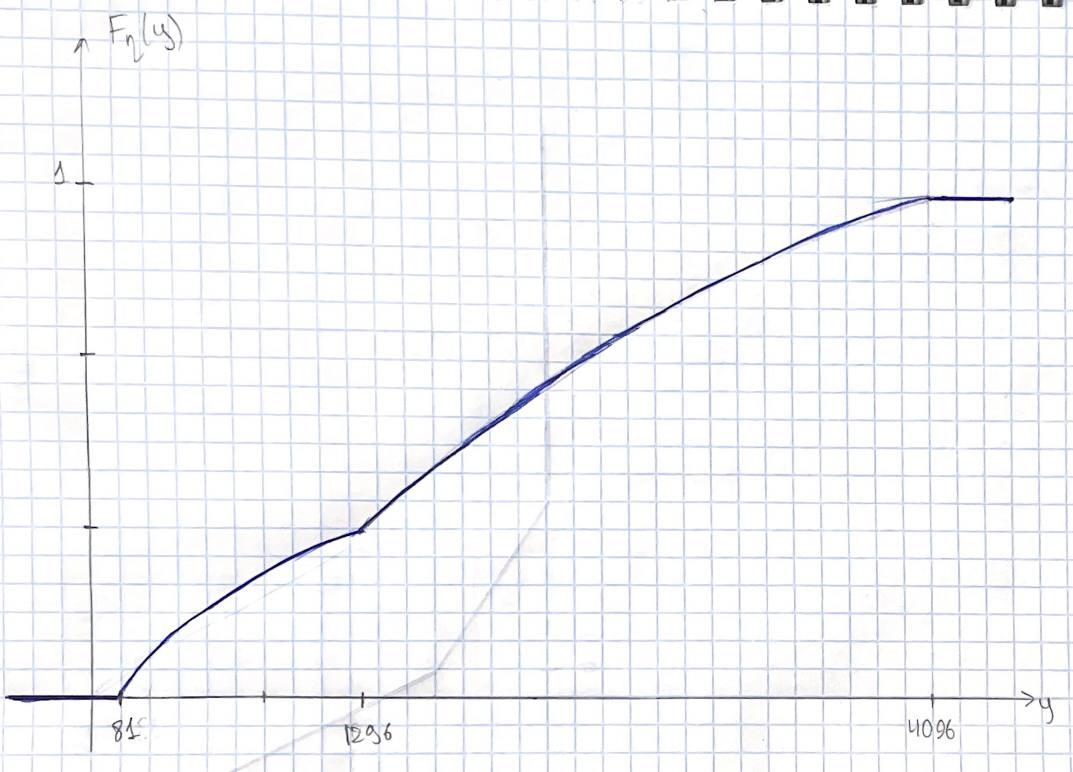
\includegraphics[width=0.5\linewidth]{4.jpg}
    \caption{}
    \label{fig:enter-label}
\end{figure}
\[
F_{\xi}(x) = \int\limits_{-\infty}^xp_{\xi}(t)dt = \begin{cases}
    0, & x\in (-\infty;3]\\
    \frac{x-3}{9}, & x\in (3; 6]\\
    \frac{x-5}{3}, & x\in (6; 8]\\
    1, & x\in (8;\infty)
\end{cases}
\]
\[
F_{\eta}(y) = \int\limits_{-\infty}^yp_{\eta}(t)dt = \begin{cases}
    0, & y\in (-\infty;81]\\
    \frac{\sqrt[4]y-3}{9}, & y\in (81; 1296]\\
    \frac{\sqrt[4]y-5}{3}, & y\in (1296; 4096]\\
    1, & y\in (4096;\infty)
\end{cases}
\]
Их графики на рисунках 3 и 4 соответственно.\\
{\it Ответ:}\\
$\Expect\xi$ = 6.1667, $\Variance\xi$ = 1.8611, $\Entropy\xi$ = 1.4648 нат\\
\end{proof}